%%%%%%%%%%%%%%%%%%%%%%%%%%%%%%%%%%%%%%%%%
% Beamer Presentation
% LaTeX Template
% Version 2.0 (March 8, 2022)
%
% This template originates from:
% https://www.LaTeXTemplates.com
%
% Author:
% Vel (vel@latextemplates.com)
%
% License:
% CC BY-NC-SA 4.0 (https://creativecommons.org/licenses/by-nc-sa/4.0/)
%
%%%%%%%%%%%%%%%%%%%%%%%%%%%%%%%%%%%%%%%%%

%----------------------------------------------------------------------------------------
%	PACKAGES AND OTHER DOCUMENT CONFIGURATIONS
%----------------------------------------------------------------------------------------
\documentclass[
	11pt, % Set the default font size, options include: 8pt, 9pt, 10pt, 11pt, 12pt, 14pt, 17pt, 20pt
	%t, % Uncomment to vertically align all slide content to the top of the slide, rather than the default centered
	%aspectratio=169, % Uncomment to set the aspect ratio to a 16:9 ratio which matches the aspect ratio of 1080p and 4K screens and projectors
]{beamer}
\usepackage{graphicx}
\usepackage[export]{adjustbox}
\usepackage{comment}
\usepackage{xcolor}
\definecolor{forestgreen(web)}{rgb}{0.13, 0.55, 0.13}
\definecolor{fuchsia}{rgb}{1.0, 0.0, 1.0}
\usepackage[export]{adjustbox}
\graphicspath{{Images/}{./}} % Specifies where to look for included images (trailing slash required)

\usepackage{booktabs} % Allows the use of \toprule, \midrule and \bottomrule for better rules in tables

%----------------------------------------------------------------------------------------
%	SELECT LAYOUT THEME
%----------------------------------------------------------------------------------------

% Beamer comes with a number of default layout themes which change the colors and layouts of slides. Below is a list of all themes available, uncomment each in turn to see what they look like.

%\usetheme{default}
%\usetheme{AnnArbor}
%\usetheme{Antibes}
%\usetheme{Bergen}
%\usetheme{Berkeley}
%\usetheme{Berlin}
%\usetheme{Boadilla}
%\usetheme{CambridgeUS}
%\usetheme{Copenhagen}
%\usetheme{Darmstadt}
%\usetheme{Dresden}
%\usetheme{Frankfurt}
%\usetheme{Goettingen}
%\usetheme{Hannover}
%\usetheme{Ilmenau}
%\usetheme{JuanLesPins}
%\usetheme{Luebeck}
\usetheme{Madrid}
%\usetheme{Malmoe}
%\usetheme{Marburg}
%\usetheme{Montpellier}
%\usetheme{PaloAlto}
%\usetheme{Pittsburgh}
%\usetheme{Rochester}
%\usetheme{Singapore}
%\usetheme{Szeged}
%\usetheme{Warsaw}

%----------------------------------------------------------------------------------------
%	SELECT COLOR THEME
%----------------------------------------------------------------------------------------

% Beamer comes with a number of color themes that can be applied to any layout theme to change its colors. Uncomment each of these in turn to see how they change the colors of your selected layout theme.

%\usecolortheme{albatross}
%\usecolortheme{beaver}
%\usecolortheme{beetle}
%\usecolortheme{crane}
%\usecolortheme{dolphin}
%\usecolortheme{dove}
%\usecolortheme{fly}
%\usecolortheme{lily}
%\usecolortheme{monarca}
%\usecolortheme{seagull}
%\usecolortheme{seahorse}
%\usecolortheme{spruce}
%\usecolortheme{whale}
%\usecolortheme{wolverine}

%----------------------------------------------------------------------------------------
%	SELECT FONT THEME & FONTS
%----------------------------------------------------------------------------------------

% Beamer comes with several font themes to easily change the fonts used in various parts of the presentation. Review the comments beside each one to decide if you would like to use it. Note that additional options can be specified for several of these font themes, consult the beamer documentation for more information.

\usefonttheme{default} % Typeset using the default sans serif font
%\usefonttheme{serif} % Typeset using the default serif font (make sure a sans font isn't being set as the default font if you use this option!)
%\usefonttheme{structurebold} % Typeset important structure text (titles, headlines, footlines, sidebar, etc) in bold
%\usefonttheme{structureitalicserif} % Typeset important structure text (titles, headlines, footlines, sidebar, etc) in italic serif
%\usefonttheme{structuresmallcapsserif} % Typeset important structure text (titles, headlines, footlines, sidebar, etc) in small caps serif

%------------------------------------------------

%\usepackage{mathptmx} % Use the Times font for serif text
\usepackage{palatino} % Use the Palatino font for serif text

\usepackage{helvet} % Use the Helvetica font for sans serif text
%\usepackage[default]{opensans} % Use the Open Sans font for sans serif text
%\usepackage[default]{FiraSans} % Use the Fira Sans font for sans serif text
%\usepackage[default]{lato} % Use the Lato font for sans serif text

%----------------------------------------------------------------------------------------
%	SELECT INNER THEME
%----------------------------------------------------------------------------------------

% Inner themes change the styling of internal slide elements, for example: bullet points, blocks, bibliography entries, title pages, theorems, etc. Uncomment each theme in turn to see what changes it makes to your presentation.

%\useinnertheme{default}
\useinnertheme{circles}
%\useinnertheme{rectangles}
%\useinnertheme{rounded}
%\useinnertheme{inmargin}

%----------------------------------------------------------------------------------------
%	SELECT OUTER THEME
%----------------------------------------------------------------------------------------

% Outer themes change the overall layout of slides, such as: header and footer lines, sidebars and slide titles. Uncomment each theme in turn to see what changes it makes to your presentation.

%\useoutertheme{default}
%\useoutertheme{infolines}
%\useoutertheme{miniframes}
%\useoutertheme{smoothbars}
%\useoutertheme{sidebar}
%\useoutertheme{split}
%\useoutertheme{shadow}
%\useoutertheme{tree}
%\useoutertheme{smoothtree}

%\setbeamertemplate{footline} % Uncomment this line to remove the footer line in all slides
%\setbeamertemplate{footline}[page number] % Uncomment this line to replace the footer line in all slides with a simple slide count

%\setbeamertemplate{navigation symbols}{} % Uncomment this line to remove the navigation symbols from the bottom of all slides

%----------------------------------------------------------------------------------------
%	PRESENTATION INFORMATION
%----------------------------------------------------------------------------------------

\title[RLC sinusoidale]{Analisi di un circuito RLC serie in regime sinusoidale} % The short title in the optional parameter appears at the bottom of every slide, the full title in the main parameter is only on the title page

\subtitle{} % Presentation subtitle, remove this command if a subtitle isn't required

\author[Davide Perniola]{Davide Perniola} % Presenter name(s), the optional parameter can contain a shortened version to appear on the bottom of every slide, while the main parameter will appear on the title slide


\date[18 Luglio, 2022]{Laboratorio di Elettromagnetismo e Ottica \\ 18 Luglio, 2022} % Presentation date or conference/meeting name, the optional parameter can contain a shortened version to appear on the bottom of every slide, while the required parameter value is output to the title slide

%----------------------------------------------------------------------------------------

\begin{document}

%----------------------------------------------------------------------------------------
%	TITLE SLIDE
%----------------------------------------------------------------------------------------

\begin{frame}
	\titlepage % Output the title slide, automatically created using the text entered in the PRESENTATION INFORMATION block above
\end{frame}

%----------------------------------------------------------------------------------------
%	TABLE OF CONTENTS SLIDE
%----------------------------------------------------------------------------------------

% The table of contents outputs the sections and subsections that appear in your presentation, specified with the standard \section and \subsection commands. You may either display all sections and subsections on one slide with \tableofcontents, or display each section at a time on subsequent slides with \tableofcontents[pausesections]. The latter is useful if you want to step through each section and mention what you will discuss.

\begin{frame}
	\frametitle{Presentazione} % Slide title, remove this command for no title
	
	\tableofcontents % Output the table of contents (all sections on one slide)
	%\tableofcontents[pausesections] % Output the table of contents (break sections up across separate slides)
\end{frame}

%----------------------------------------------------------------------------------------
%	PRESENTATION BODY SLIDES
%----------------------------------------------------------------------------------------

\section{Apparato sperimentale} % Sections are added in order to organize your presentation into discrete blocks, all sections and subsections are automatically output to the table of contents as an overview of the talk but NOT output in the presentation as separate slides
	
%------------------------------------------------

\subsection{Circuito}

\begin{frame}
	\frametitle{Circuito}
	\begin{figure}[ht]
		\begin{minipage}[c][3cm]{0.5\linewidth}
		\centering
		\includegraphics[%scale=1
						 width=1\linewidth, valign=t]{Circuito.png}
		
		\end{minipage}%
		\hspace{1cm}
		\begin{minipage}[c][8cm]{0.35\linewidth}
			$R_I=50\Omega$ \\ \\
			$R=(330.0\pm0.3)\Omega$ \\ \\$R_L=(34.5\pm0.1)\Omega$\\ \\$L=(10.3\pm0.1)mH$ \\ \\ $C=(45.5\pm0.4)nF$
		\end{minipage}
		\end{figure}
	
\end{frame}

%-----------------------------------------------

%------------------------------------------------

\subsection{Acquisizione e analisi}

\begin{frame}
	\frametitle{Acquisizione e analisi}
	\begin{figure}[ht]
		\begin{minipage}[c][3cm]{0.5\linewidth}
		\centering
		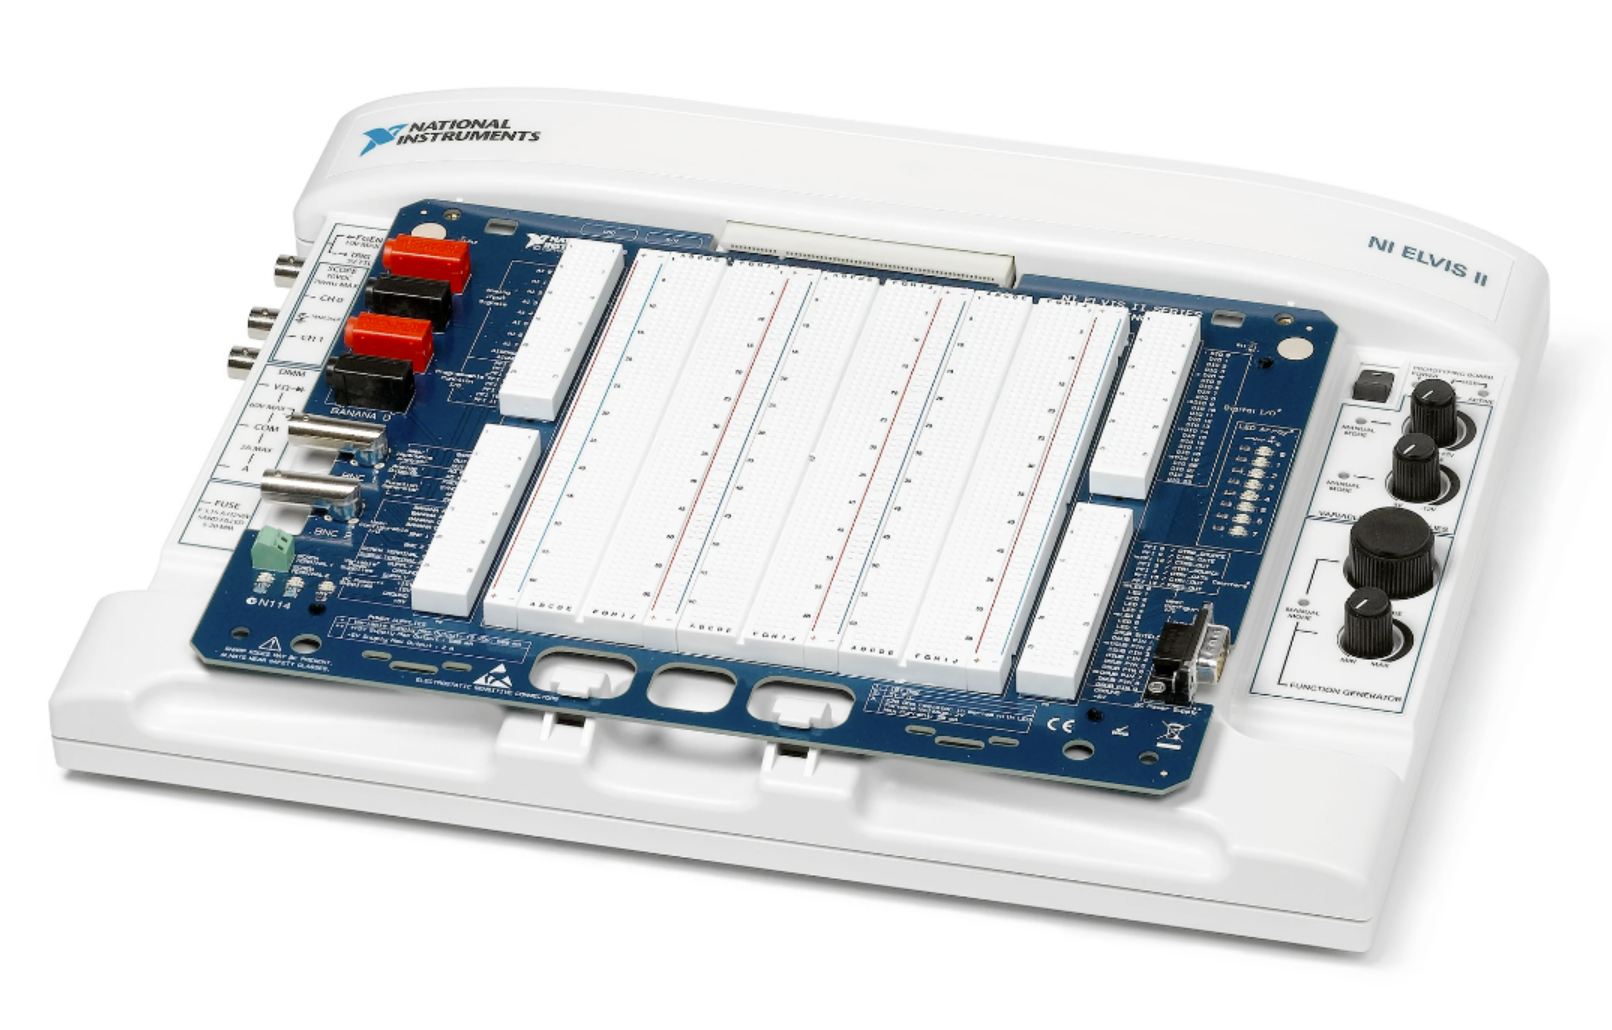
\includegraphics[%scale=1
						 width=1\linewidth, valign=t]{elvisII.png}
		
		\end{minipage}%
		\hspace{1cm}
		\begin{minipage}[c][8cm]{0.35\linewidth}
			\begin{itemize}
				\setlength\itemsep{2cm}
				\item Scheda Elvis II
				\item Programma scritto in LabVIEW
				\item Dati elaborati con il softwere ROOT
			\end{itemize}
		\end{minipage}
		\end{figure}
	
\end{frame}

\subsection{Svolgimento}

\begin{frame}
	\frametitle{Svolgimento}
	\begin{figure}[ht]
		\begin{minipage}[c][3cm]{0.28\linewidth}
		\centering
		\includegraphics[%scale=1
						 width=1\linewidth, valign=t]{Circuito.png}
		
		\end{minipage}%
		\hspace{0.5cm} 
		\begin{minipage}[c][6cm][t]{0.605\linewidth}
			$V(t)=V_{0}\cos{wt} $ \\ \\ \\
			$i(t)=\frac{V_{0}}{\sqrt{R^2+(wL-\frac{1}{wC})^2}}\cos{[wt+(\arctan{\frac{1-w^2LC}{wRC}})]}$ \\ \\ \\
			$R(w)=\frac{1}{1+q^2(\frac{w_0}{w}-\frac{w}{w_0})}$ \quad $q=\frac{w_0L}{R}=\frac{1}{R}\sqrt{\frac{L}{C}}$ \\ \\ \\
			$w_0=\frac{1}{\sqrt{LC}}$ \\ \\
			Nel caso del nostro circuito \\ \\
			$q\approx 1.5$ \qquad $f_0=(7351\pm68)Hz$
 
		\end{minipage}
		\end{figure}
	
	
\end{frame}
%------------------------------------------------

%------------------------------------------------

\section{Risultati}

\subsection{Studio qualitativo}

\begin{frame}
	\frametitle{Studio qualitativo: $4000Hz$}
	
		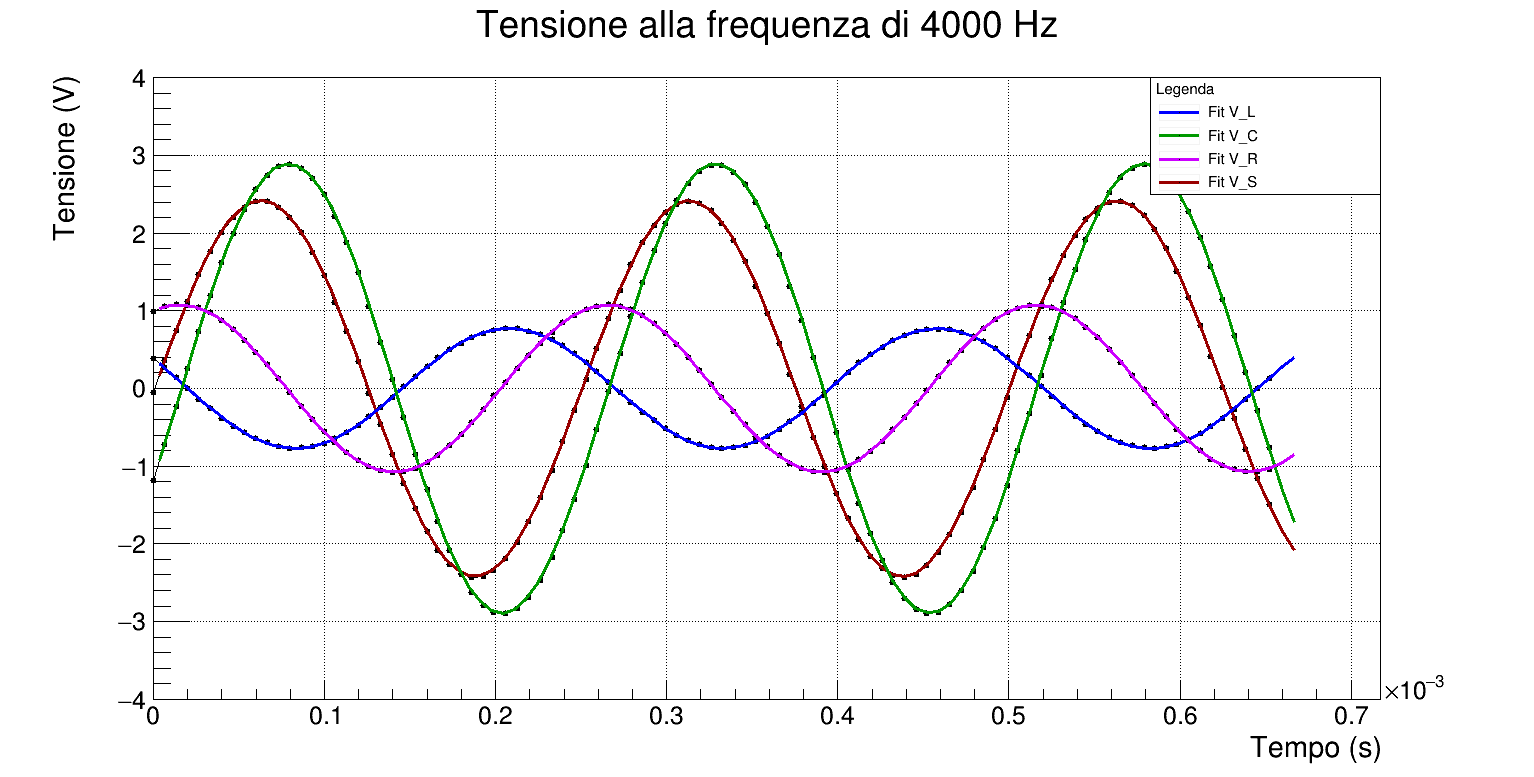
\includegraphics[%scale=1
						 width=1.06\linewidth]{FitFMin.png}
		
		
\end{frame}

\begin{frame}
	\frametitle{Studio qualitativo: $f_0$}
	
		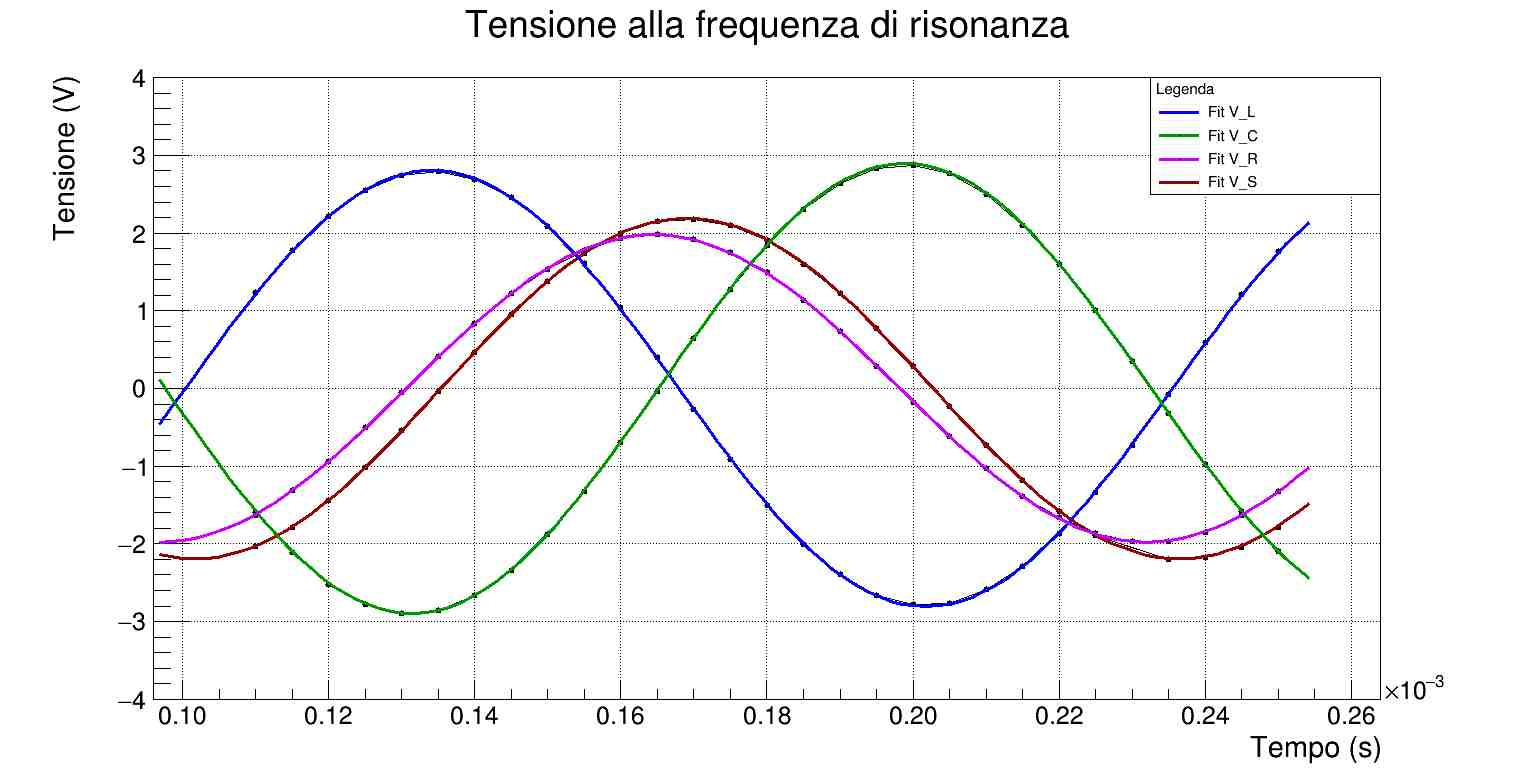
\includegraphics[%scale=1
						 width=1.06\linewidth]{FitF0.jpg}
		
		
\end{frame}

\begin{frame}
	\frametitle{Studio qualitativo: $10000Hz$}
	
		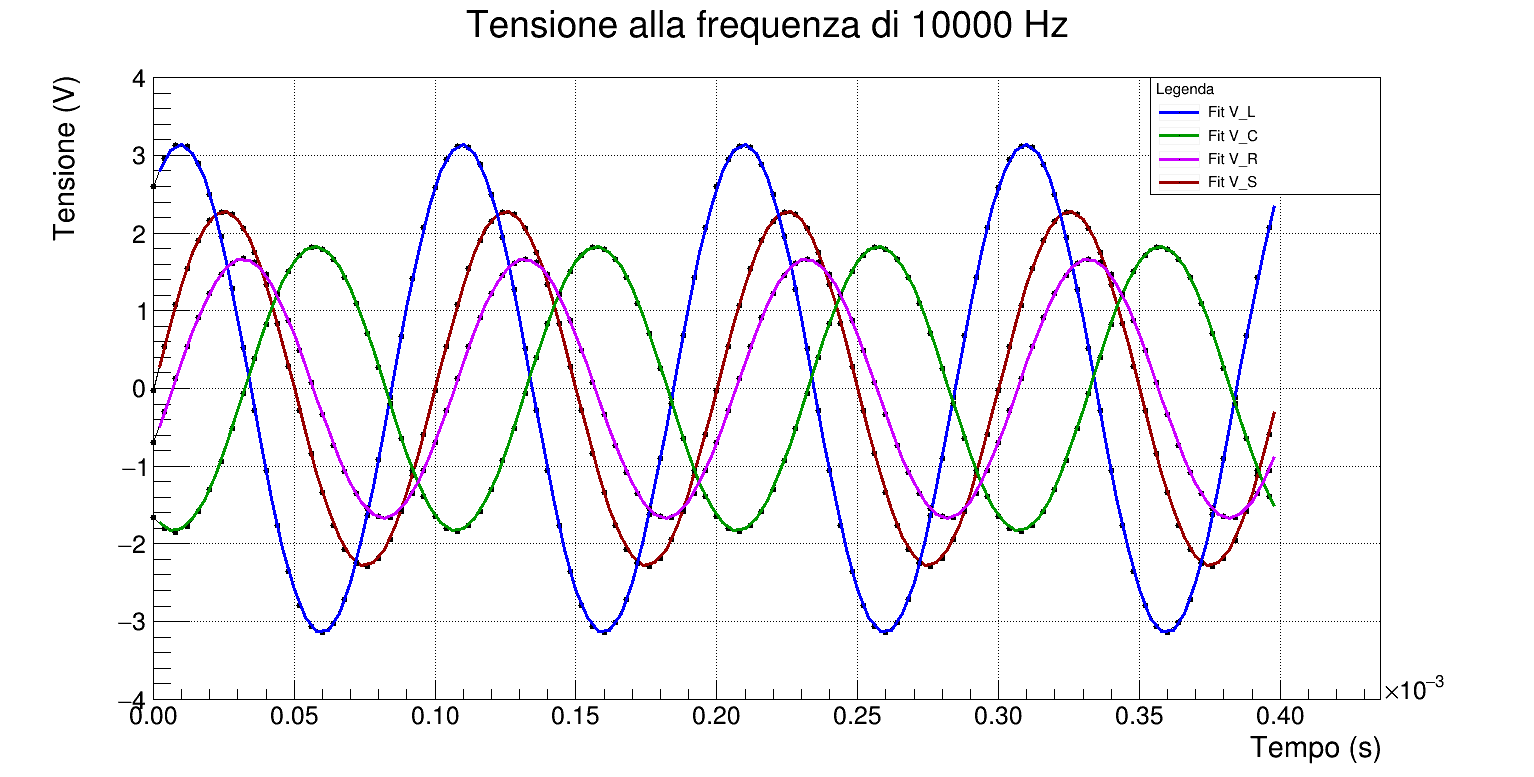
\includegraphics[%scale=1
						 width=1.06\linewidth]{FitFMag.png}
		
		
\end{frame}

\subsection{Analisi dell'ampiezza}
\begin{frame}
	\frametitle{Analisi dell'ampiezza}
	\framesubtitle{} % Optional subtitle
	\begin{figure}[ht]
		\begin{minipage}[c][3cm]{0.65\linewidth}
		\centering
		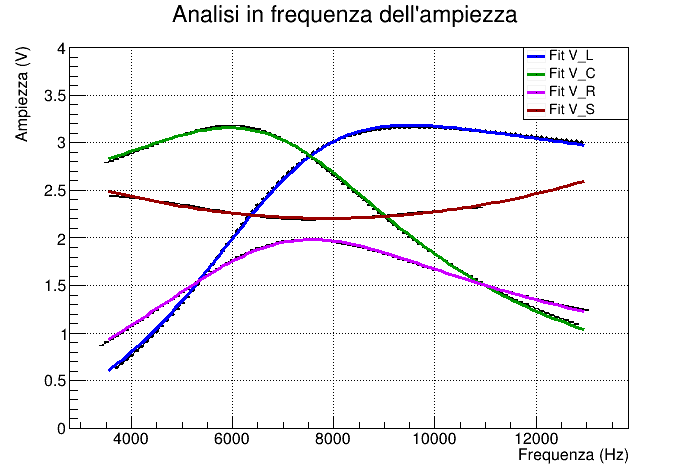
\includegraphics[%scale=1
						 width=1\linewidth, valign=t]{AmpFreq.png}
		
		\end{minipage}%
		\hspace{0.cm}
		\begin{minipage}[c][6cm][t]{0.33\linewidth}
			$ \textcolor{fuchsia}{A_R(w) =\frac{V_{0}R}{\sqrt{R^2+(wL-\frac{1}{wC})^2}}}$ \\ \\ \\ \\ \\
			$ \textcolor{blue}{A_L(w) =\frac{V_{0}wL}{\sqrt{R^2+(wL-\frac{1}{wC})^2}}}$ \\ \\ \\\\ \\
			$ \textcolor{forestgreen(web)}{A_C(w) =\frac{\frac{V_{0}}{wC}}{\sqrt{R^2+(wL-\frac{1}{wC})^2}}}$ 
		\end{minipage}
		$f_0s=(7562\pm5)Hz$
		\end{figure}
	
\end{frame}

\subsection{Analisi della fase}
\begin{frame}
	\frametitle{Analisi della fase}
	\framesubtitle{} % Optional subtitle
	\begin{figure}[ht]
		\begin{minipage}[c][3cm]{0.61\linewidth}
		\centering
		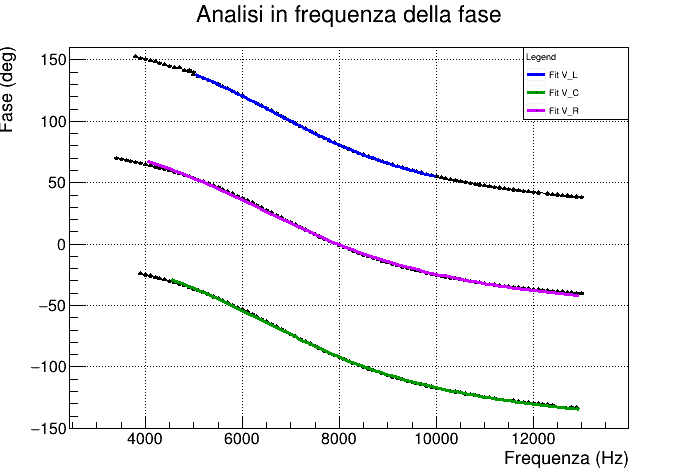
\includegraphics[%scale=1
						 width=1\linewidth, valign=t]{FaseFreq2.png}
		
		\end{minipage}%
		\hspace{0cm}
		\begin{minipage}[c][6cm][t]{0.381\linewidth}
			$\textcolor{fuchsia}{\Phi_R(w)=\arctan{\frac{1-w^2LC}{wRC}}}$ \\ \\ \\ \\ \\ 
			$\textcolor{blue}{\Phi_L(w)=\arctan{(\frac{1-w^2LC}{wRC})}+\frac{\pi}{2}}$ \\ \\ \\ \\ \\ 
			$\textcolor{forestgreen(web)}{\Phi_C(w)=\arctan{(\frac{1-w^2LC}{wRC})}-\frac{\pi}{2}}$ \\ \\ \\ \\\\

		\end{minipage}
		\end{figure}
	
\end{frame}

%----------------------------------------------
%------------------------------------------------

\section{Conclusioni}

\begin{frame}
	\frametitle{Conclusioni: problematiche e possibili soluzioni}
	
	\begin{definition}
		A \alert{prime number} is a number that has exactly two divisors.
	\end{definition}
	
	\smallskip % Vertical whitespace
	
	\begin{example}
		\begin{itemize}
			\item 2 is prime (two divisors: 1 and 2).
			\item 3 is prime (two divisors: 1 and 3).
			\item 4 is not prime (\alert{three} divisors: 1, 2, and 4).
		\end{itemize}
	\end{example}
	
	\smallskip % Vertical whitespace
	
	You can also use the \texttt{theorem}, \texttt{lemma}, \texttt{proof} and \texttt{corollary} environments.
\end{frame}

%------------------------------------------------


%------------------------------------------------


%------------------------------------------------


%------------------------------------------------


%------------------------------------------------



%----------------------------------------------------------------------------------------
%	ACKNOWLEDGMENTS SLIDE
%----------------------------------------------------------------------------------------
\begin{frame}
	\frametitle{Analisi dati}
	\framesubtitle{} % Optional subtitle
	
	\begin{columns}[c] % The "c" option specifies centered vertical alignment while the "t" option is used for top vertical alignment
		\begin{column}{0.45\textwidth} % Left column width
			\textbf{Heading}
			\begin{enumerate}
				\item Statement
				\item Explanation
				\item Example
			\end{enumerate}
		\end{column}
		\begin{column}{0.5\textwidth} % Right column width
			Lorem ipsum dolor sit amet, consectetur adipiscing elit. Integer lectus nisl, ultricies in feugiat rutrum, porttitor sit amet augue. Aliquam ut tortor mauris. Sed volutpat ante purus, quis accumsan dolor.
		\end{column}
	\end{columns}
\end{frame}


%----------------------------------------------------------------------------------------
%	CLOSING SLIDE
%----------------------------------------------------------------------------------------

\begin{frame}[plain] % The optional argument 'plain' hides the headline and footline
	\begin{center}
		{\Huge The End}
		
		\bigskip\bigskip % Vertical whitespace
		
		{\LARGE Questions? Comments?}
	\end{center}
\end{frame}

%----------------------------------------------------------------------------------------

\end{document} 